\documentclass{beamer}
\mode<presentation>
 \usetheme{CambridgeUS}


\title[Pythonic Parsing with Pyparsing]{Pythonic Parsing with Pyparsing}

\author[Dr Andrew Lawrence]{Dr Andrew Lawrence}
\date[PyCon UK, 17 September 2018]{PyCon UK 2018\\[1em]  Cardiff, 17 September 2018}

\usepackage{tikz}
\usepackage{graphicx}
\usetikzlibrary{shapes}
\usetikzlibrary{positioning}
\usetikzlibrary{arrows}
\usetikzlibrary{automata}
\usepackage{tikz-uml}
\usepackage{verbatim}
\newcommand{\Red}{\mathbf{Red}}
\usepackage[nounderscore]{syntax}
\usepackage[linguistics]{forest}
%\usepackage{forest}

\newtheorem{mydef}{Definition}
\newtheorem{myremark}{Remark}
\newcommand{\ednote}[1]{{\bf #1}}
\newcommand{\fig}[1]{Fig.~\ref{fig:#1}}
\newcommand{\Val}{{\rm Val}}
\newcommand{\unprime}{{\rm unprime}}
\newcommand{\Vars}{{\rm Vars}}
\definecolor{bottomcol}{RGB}{222,222,222}


\usepackage[T1]{fontenc}
\usepackage{lmodern}
\newcommand*{\escape}[1]{\texttt{\textbackslash#1}}

\begin{document}
\tikzstyle{class}=[
    rectangle,
    draw=black,
    text centered,
    anchor=north,
    text=black,
    text width=3cm,
    shading=axis,
    bottom color=bottomcol,top color=white,shading angle=45]


\begin{frame}
  \titlepage
\end{frame}

\begin{frame}
\frametitle{Who Am I?}
\begin{itemize}
\item Software Engineer
\pause
\item Previously, I did a PhD looking at automatic formal verification of train control systems
\pause
\item First Pycon
\pause
\item First workshop
\end{itemize}
\end{frame}

\begin{frame}

\frametitle{Workshop Overview}

\medskip
This workshop aims to give an introduction to parsing using the Pyparsing library
%\pause

\medskip

Overview:

\begin{itemize}
  \item \underline{Part I:} Parsing Introduction
  \item \underline{Part II:} Pyparsing Basics
  \item \underline{Part III:} Exercise 1: Dice Rolling
  \item \underline{Part IV:} Intermediate Pyparsing
  \item \underline{Part V:} Exercise 2: JSON Parser
  \item \underline{Part VI:} Advanced Pyparsing
\end{itemize}
\end{frame}

\begin{frame}

\frametitle{Prerequisites}
I am assuming that you have \textbf{Python 3} and \textbf{git} installed. You can get the workshop examples from Github:
\begin{center}
\textit{git clone https://github.com/andrewjlawrence/pyparsingworkshop.git}
\end{center}
\bigskip
You also need to install Pyparsing. 
\begin{center}
\textit{pip install pyparsing}
\end{center}
\end{frame}

\section{Parsing Introduction}

%\begin{frame}
%\begin{center}
%{\Large ERTMS -- what it is}
%\end{center}

%\end{frame}


\tikzstyle{block} = [rectangle, draw, fill=blue!20, 
    text width=5em, text centered, rounded corners, minimum height=4em]
\tikzstyle{line} = [draw, -latex']
\tikzstyle{cloud} = [draw, ellipse,fill=red!20,
    minimum height=2em]


\begin{frame}
\frametitle{Why do we need parsers?}
The world is full of textual data in structured human readable formats. \\
\begin{itemize}
\item XML
\item JSON
\item other propriety formats...
\end{itemize}
\bigskip
The problem here is getting computers to understand this data.
\end{frame}

\begin{frame}[fragile]
\frametitle{Why do we need parsers?}
\begin{verbatim}
  <customer id="cust0921">
    <first-name>Andrew</first-name>
    <last-name>Lawrence</last-name>
    <address>
      <street>Langley Park</street>
      <city>Chippenham</city>
      <county>Wiltshire</county>
      <postcode>SN122BL</postcode>
    </address>
  </customer>
\end{verbatim}


\end{frame}

\begin{frame}
\frametitle{What is a parser?}
Typically parsing involves 3 stages:
\medskip
\begin{description}
\item[Lexical Analysis] Break the string down into \textbf{tokens}

\item[Syntactic Analysis] Construct a \textbf{syntax tree} based on some grammar

\item[Semantic Interpretation] Do something based on the syntax tree
\end{description}

\end{frame}
    

\begin{frame}
\frametitle{What is a parser?}
\begin{center}
\scalebox{0.8}
{
\begin{tikzpicture}[node distance = 2cm]
    % Place nodes
    \node [cloud] (init) {Source String};
    \node [block, below of=init] (lex) {Lexical Analysis};
    \node [cloud, below of=lex] (tokens) {Tokens};
    \node [block, below of=tokens] (syntax) {Syntactic Analysis};
    \node [cloud, below of=syntax] (parsetree) {Syntax Tree};
    % Draw edges
    \path [line] (init) -- (lex);
    \path [line] (lex) -- (tokens);
    \path [line] (tokens) -- (syntax);
    \path [line] (syntax) -- (parsetree);
\end{tikzpicture}
}
\end{center}
\end{frame}

\begin{frame}
\frametitle{What is a Grammar?}

A \textbf{grammar} is a set of rules that describes the structure of text. \\
\bigskip
It specifies the syntax that should be accepted by the parser.
\end{frame}


\begin{frame}[fragile]
\frametitle{Backus-Naur Form (BNF)}
A Backus-Naur form (BNF) is metasyntax notation for describing grammars.

\begin{center}
  \begin{tabular}{ | c | c | }
    \hline
    element type & description \\ \hline\hline
    $<\mathrm{non terminals}>$ & non terminal symbols  \\ \hline
    \textbf{terminals} & terminal symbols  \\ \hline
    $|$ & choice  \\ \hline
    ::= & replaced-by  \\ 
    \hline
  \end{tabular}
\end{center}

\end{frame}

\begin{frame}[fragile]
\frametitle{Arithmetic Example Grammar}
\begin{grammar}
<sum> ::= <sum> $\mathbf{+}$ <product> | <product>

<product> ::= <product> $\mathbf{*}$ <value> | <value>

<value> ::= <int> | \textit{id}

<int> ::= <unsignedint> | $\mathbf{-}$<unsignedint>

<unsignedint> ::= <digit> | <unsignedint><digit>

<digit> ::= $\mathbf{0}$ | $\mathbf{1}$ | $\mathbf{2}$ | $\mathbf{3}$ | $\mathbf{4}$ | $\mathbf{5}$ | $\mathbf{6}$ | $\mathbf{7}$ | $\mathbf{8}$ | $\mathbf{9}$
 \end{grammar}
\end{frame}


\begin{frame}
\frametitle{Regular Expressions}
A \textit{regular expression} is a syntactic notation for defining textual patterns. \\
\bigskip
Example: \texttt{a|b*} denotes ${\{ \epsilon, "a", "b", "bb", "bbb", \ldots \}}$ \\
\bigskip
I won't go into further detail about how these work but beaware that they exist.
\end{frame}


\begin{frame}[fragile]
\frametitle{BNF Extensions}
There are a number of extensions to BNF. One common approach, as seen in extended Backus-Naur form is to use operations from regular expressions such as:

\begin{description}
\item[*]  - Match the preceeding element zero or more times. Often called the \underline{\textbf{Kleene Star}}.
\item[+]  - Match the preceeding element one or more times
\end{description}

\end{frame}



\begin{frame}
\frametitle{Types of Parsers}
\begin{center}
\begin{tikzpicture}[post/.style={->,shorten >=1pt,>=stealth',semithick}] 
\umlsimpleclass{Parser} 
\umlsimpleclass[x=-2, y=-3]{Top down} 
\umlsimpleclass[x=2, y=-3]{Bottom up}
\umlVHVinherit{Top down}{Parser} 
\umlVHVinherit{Bottom up}{Parser} 
\end{tikzpicture}
\end{center}
\end{frame}



\tikzset{
    invisible/.style={opacity=0,text opacity=0},
    visible on/.style={alt=#1{}{invisible}},
    alt/.code args={<#1>#2#3}{%
      \alt<#1>{\pgfkeysalso{#2}}{\pgfkeysalso{#3}} % \pgfkeysalso doesn't change the path
    },
}
\forestset{
  visible on/.style={
    for current and ancestors={
      /tikz/visible on={#1},
      edge={/tikz/visible on={#1}}}}}

\begin{frame}
\frametitle{Example Parse Tree}
\begin{center}
\scalebox{0.8} {
\begin{forest}
  for tree={
    if n children=0{
      font=\itshape,
      tier=terminal,
      l sep=20pt,
      minimum width=1.8cm
    }{},
  }
[sum
  [sum
    [product
      [product
        [value
          [id
            [$x$]
          ]
        ]
      ]
      [$*$]
      [value
        [int 
          [$2$]
        ]
      ]
    ]
  ]
  [$+$]
  [product 
    [value
      [int
        [$1$]
      ]
    ]
  ]
]
\end{forest}
}
\end{center}
\end{frame}

\begin{frame}
\frametitle{Bottom Up (LR) Parse}
\begin{center}
\scalebox{0.8} {
\begin{forest}
  for tree={
    if n children=0{
      font=\itshape,
      tier=terminal,
      l sep=20pt,
      minimum width=1.8cm
    }{},
  }
[sum (13), , visible on=<13->
  [sum (8), , visible on=<8->
    [product (7), visible on=<7->
      [product (3), visible on=<3->
        [value (2), visible on=<2->
          [id (1), visible on=<1->
            [$x$, visible on=<1->]
          ]
        ]
      ]
      [$\overset{(4)}{*}$, visible on=<4->]
      [value (6), visible on=<6->
        [int (5), visible on=<5->
          [$2$, visible on=<5->]
        ]
      ]
    ]
  ]
  [$\overset{(9)}{+}$, , visible on=<9->]
  [product (12) , visible on=<12->
    [value (11), visible on=<11->
      [int (10),  visible on=<10->
        [$1$,  visible on=<10->]
      ]
    ]
  ]
]
\end{forest}
}
\end{center}
\end{frame}
\tikzset{
    invisible/.style={opacity=0,text opacity=0},
    visible on/.style={alt=#1{}{invisible}},
    alt/.code args={<#1>#2#3}{%
      \alt<#1>{\pgfkeysalso{#2}}{\pgfkeysalso{#3}} % \pgfkeysalso doesn't change the path
    },
}
\forestset{
  visible on/.style={
    for tree={
      /tikz/visible on={#1},
      edge+={/tikz/visible on={#1}}}}}


\begin{frame}
\frametitle{Top Down Parse}
\begin{center}
\scalebox{0.8} {
\begin{forest}
  for tree={
    if n children=0{
      font=\itshape,
      tier=terminal,
      l sep=20pt,
      minimum width=1.8cm
    }{},
  }
[sum (1), visible on=<1->
  [sum (2), visible on=<2->
    [product (3), visible on=<3->
      [product (4), visible on=<4->
        [value (5), visible on=<5->
          [id (6), visible on=<6->
            [$x$, visible on=<6->]
          ]
        ]
      ]
      [$\overset{(7)}{*}$, visible on=<7->]
      [value (8), visible on=<8->
        [int (9), visible on=<9->
          [$2$, visible on=<9->]
        ]
      ]
    ]
  ]
  [$\overset{(10)}{+}$, visible on=<10->]
  [product (11), visible on=<11->
    [value (12), visible on=<12->
      [int (13), visible on=<13->
        [$1$, visible on=<13->]
      ]
    ]
  ]
]
\end{forest}
}
\end{center}
\end{frame}


%\begin{frame}
%\frametitle{More detailed description of recursive decent parsing}
%\end{frame}

\begin{frame}[fragile]
\frametitle{Why Are Regular Expressions Bad You Ask?}
Below is part of a regex for validating RFC822 email addresses.
\begin{verbatim}
(?:(?:\\r\\n)?[ \\t])*(?:(?:(?:[^()<>@,;:\\\\".\\[\\]
 \\000-\\031]+(?:(?:(?:\\r\\n)?[ \\t])+|\\Z|
(?=[\\["()<>@,;:\\\\".\\[\\]]))|"(?:[^\\\\"\r\\\\]|\\\\.|
(?:(?:\\r\\n)?[ \\t]))*"(?:(?:\\r\\n)?[ \\t])*)
(?:\\.(?:(?:\\r\\n)?[ \\t])
*(?:[^()<>@,;:\\\\".\\[\\] \\000-\\031]+
(?:(?:(?:\\r\\n)?[ \\t])+|\\Z|
(?=[\\["()<>@,;:\\\\".\\[\\]]))|"
(?:[^\\"\r\\\\]|\\\\.|(?:(?:\\r\\n)?[ \t]))
*"(?:(?:\\r\\n)?[ \\t])*))*@(?:(?:\\r\\n)?[ \\t])*
\end{verbatim}
The full regex is 6.2KB in size.

\end{frame}


\begin{frame}[fragile]
\frametitle{Why Are Regular Expressions Bad You Ask?}
Why are regular expressions bad?

\begin{enumerate}
\pause
\item Difficult to read
\pause
\item Hard to maintain - Write only
\pause
\item Different standards exist
\end{enumerate}

\end{frame}

\section{Pyparsing Basics}

\begin{frame}
\frametitle{Pyparsing Overview}
Pyparsing is a recursive decent parser framework for the Python programming language. \\
\medskip
Created by Paul McGuire in 2003. \\
\medskip
Follows the parser combinator approach to parsing.
\end{frame}

\begin{frame}
\frametitle{Parser Combinator Approach}
You build your parser by combining other parsers.
$$Parser_3 = Parser_1 + Parser_2$$
\end{frame}

\begin{frame}
\frametitle{Pyparsing Advantages}

\textbf{\underline{Comprehensive framework}} - Contains many predefined parsers. \\
\medskip
\textbf{\underline{Powerful}} - More so than regular expressions (Parsing expression grammar vs regular grammar).\\
\bigskip
\textbf{\underline{High-level}} - Lets us define parsers using a BNF style notation.
\end{frame}

\begin{frame}
\frametitle{Chomsky Hierarchy}
Noam Chomsky did a lot of foundational research in formal language theory in the 1950s

$$REG \subset CF \subset CS \subset RE$$

\underline{\textbf{REG} Regular languages} - those defined by regular expression \\ \medskip
\underline{\textbf{CF} Context-free languages} - no context in the syntactic rules \\ \medskip
\underline{\textbf{CS} Context-sensitive languages} - can have context in syntactic rules \\ \medskip
\underline{\textbf{RE} Recursively enumerable languages} - all languages that can be parsed on a computer
\end{frame}

\begin{frame}
\frametitle{Parsing Expression Grammar}
Pyparsing utilizes \textit{Parsing Expression Grammars} which have been around since 2004. \\
\medskip
Very similar to context-free languages but the choice operator $|$ is deterministic.
\end{frame}

\begin{frame}
\frametitle{Pyparsing is Pythonic}
Consider the below points from "The Zen of Python": \\
\bigskip
\begin{itemize}
\item Beautiful is better than ugly.
\item Explicit is better than implicit.
\item Simple is better than complex.
\item Readability counts.
\end{itemize}
\end{frame}

\begin{frame}
\frametitle{The Zen of Pyparsing (by Paul McGuire) Part 1}
Don't clutter up the parser grammar with whitespace, just handle it! (likewise for comments) \\
\bigskip
Grammars must tolerate change, as grammar evolves or input text becomes more challenging. \\
\bigskip
Grammars do not have to be exhaustive to be useful. 
\end{frame}

\begin{frame}
\frametitle{The Zen of Pyparsing (by Paul McGuire) Part 2}
Simple grammars can return lists; complex grammars need named results. \\
\bigskip
Class names are easier to read and understand than specialized typography. \\
\bigskip
Parsers can (and sometimes should) do more than tokenize.
\end{frame}


\begin{frame}
\frametitle{Arthmetic Example in Pyparsing}
See arthmetic example \textbf{sum.py}
\end{frame}


\begin{frame}[fragile]
\frametitle{Getting Started}
Loading the module inside a Python script can be done like so
\begin{verbatim}
import pyparsing as pp
\end{verbatim}
\bigskip
You can then define some parser and call either parseString or scanString.
\begin{verbatim}
myparser.parseString("Somestring")
\end{verbatim}
\end{frame}


\begin{frame}
\frametitle{Parser Element}
The basic building block from which all other parsers are built
\begin{center}
\begin{tikzpicture}[post/.style={->,shorten >=1pt,>=stealth',semithick}] 
\umlsimpleclass{object} 
\umlclass[y=-3]{ParserElement}{}{parseString(self, instring) : ParseResults \\
	runTests(self, tests)
}
\umlVHVinherit{ParserElement}{object} 
\end{tikzpicture}
\end{center}
\end{frame}



\begin{frame}[fragile]
\frametitle{parseString}
Applying the parser to a string is done using the \texttt{parseString} method.

\begin{verbatim}
sum.parseString("4 + 2 * 4")

=>

['4', '+', '2', '*', '4']
\end{verbatim}
It should be noted that whitespace is skipped by default.
\end{frame}


\begin{frame}[fragile]
\frametitle{runTests}
It is possible to run some simple tests using the \texttt{runTests} method.

\begin{verbatim}
tests = """
    1+2
    1+3+7
    -1*43
    -1+16*4
    """
sum.runTests(tests)
\end{verbatim}
The results will either show that the parse succeeded or where it failed. \\
\medskip
It is always advisable to write unit tests for real application development.
\end{frame}


\begin{frame}
\frametitle{Pyparsing Basics: Defining Tokens}
\begin{center}
\begin{tikzpicture}[post/.style={->,shorten >=1pt,>=stealth',semithick}] 
\umlsimpleclass{object} 
\umlsimpleclass[y=-2]{ParserElement}
\umlsimpleclass[y=-4]{Token}
\umlsimpleclass[x=-3, y=-6 ]{Literal}
\umlsimpleclass[x=0, y=-6 ]{Word}
\umlsimpleclass[x=3, y=-6 ]{Keyword}
\umlVHVinherit{ParserElement}{object} 
\umlVHVinherit{Token}{ParserElement} 
\umlVHVinherit{Literal}{Token} 
\umlVHVinherit{Word}{Token} 
\umlVHVinherit{Keyword}{Token} 
\end{tikzpicture}
\end{center}
\end{frame}



\begin{frame}[fragile]
\frametitle{Pyparsing Basics: Literal}
\texttt{Literal} can be used to exactly match a specified string
\begin{verbatim}
   Literal('blah').parseString('blah')  
        # -> ['blah']
   Literal('blah').parseString('blahfooblah')  
        # -> ['blah']
   Literal('blah').parseString('bla')  
        # -> Exception: Expected "blah"
\end{verbatim}
There is also a \texttt{CaselessLiteral} token class for case-insensitive matching.
\end{frame}

\begin{frame}[fragile]
 \frametitle{Pyparsing Basics: Word}
Token to match a word based on a provided character set. \\ 
\bigskip
The following grammar 
\begin{grammar}
<abstring> ::= ($\mathbf{a}$ | $\mathbf{b}$ | $\mathbf{A}$ | $\mathbf{B}$)*
 \end{grammar} 
\bigskip
is equivalent to this Python code
\begin{verbatim}
abstring = pp.Word("abAB")
 \end{verbatim}

\end{frame}


\begin{frame}[fragile]
 \frametitle{Pyparsing Basics: Word}
There are several helper strings for defining words \\ 
\begin{center}
  \begin{tabular}{ | c | c | }
    \hline
    helper string & description \\ \hline\hline
    alphas & alphabetic characters  \\ \hline
    nums & numbers \\ \hline
    alphanums & alphabetic characters + numbers  \\ \hline
    hexnums & hexidecimal numbers  \\ \hline
    alphas8bit & alphabetic characters in ASCII range 128-255 \\ \hline
    punc8bit & non-alphabetic characters in ASCII range 128-255 \\ \hline
    printables & any non-whitespace character \\
  \hline
  \end{tabular}
\end{center}

\end{frame}

\begin{frame}[fragile]
 \frametitle{Pyparsing Basics: Word}
In our arthmetic example we define \texttt{unsignedint} using the \texttt{Word} Token.
\begin{verbatim}
unsignedint = pp.Word(pp.nums)

unsignedint.parseString("123")
        # => ['123']	

unsignedint.parseString("abc")
# => pyparsing.ParseException: Expected W:(0123...)	
\end{verbatim}
See example \textbf{integer-withoutnames.py}
\end{frame}

\begin{frame}
\frametitle{Pyparsing Basics: Word Length}
Word has some helpful parameters for lengths.

\begin{description}
\item[exact] Match with exactly this length
\item[max] Match with a maximum length
\item[min] Match with a minimum length
\end{description}
\bigskip

See example \textbf{digit.py}
\end{frame}

\begin{frame}[fragile]
\frametitle{Pyparsing Basics: ParseResults}
\begin{center}
\begin{tikzpicture}[post/.style={->,shorten >=1pt,>=stealth',semithick}] 
\umlsimpleclass{object} 
\umlclass[y=-3]{ParseResults}{}{asList()  \\
	asDict() \\
        getName()
}
\umlVHVinherit{ParserElement}{object} 
\end{tikzpicture}
\end{center}
\end{frame}


\begin{frame}[fragile]
\frametitle{Pyparsing Basics: Result Names}
It is possible to label results using a name
\begin{verbatim}
unsignedint = \
 pp.Word(pp.nums).setResultsName('Unsigned Integer')

unsignedint.runTests("""
        1
""") 
  =>
1
['1']
- Unsigned Integer: '1'
\end{verbatim}
See example \textbf{integer-withnames-v1.py}
\end{frame}


\begin{frame}[fragile]
\frametitle{Pyparsing Basics: Keyword}
The Keyword parser can be used to match works that must be seperated by white space.
\begin{verbatim}
print(pp.Keyword("if").parseString("if (1 + 1 = 2)"))
=>
	["if"]
print(pp.Keyword("if").parseString("ifAndOnlyIf"))
=>
 	ParseException
\end{verbatim}
See example \textbf{ifstatement.py}
\end{frame}


\begin{frame}
\frametitle{Pyparsing Basics: ParseExpressions}

\begin{center}
\begin{tikzpicture}[post/.style={->,shorten >=1pt,>=stealth',semithick}] 
\umlsimpleclass{object} 
\umlsimpleclass[y=-2]{ParserElement}
\umlsimpleclass[y=-4]{ParseExpression}
\umlsimpleclass[x=-4, y=-6 ]{And}
\umlsimpleclass[x=-1.5, y=-6 ]{Each}
\umlsimpleclass[x=1.5, y=-6 ]{MatchFirst}
\umlsimpleclass[x=4, y=-6 ]{Or}
\umlVHVinherit{ParserElement}{object} 
\umlVHVinherit{ParseExpression}{ParserElement} 
\umlVHVinherit{And}{ParseExpression} 
\umlVHVinherit{Each}{ParseExpression} 
\umlVHVinherit{MatchFirst}{ParseExpression} 
\umlVHVinherit{Or}{ParseExpression} 

\end{tikzpicture}
\end{center}

\end{frame}


\begin{frame}[fragile]
\frametitle{Pyparsing Basics: And}
The \texttt{And} parse expression, written infix as \texttt{+}, requires that the given ParseExpressions are found in order.

\begin{verbatim} 
pp.Literal("-") + unsignedint
\end{verbatim}

or as prefix notation
\begin{verbatim} 
pp.And([pp.Literal("-"), unsignedint])
\end{verbatim}

\end{frame}



\begin{frame}[fragile]
\frametitle{Pyparsing Basics: Each}
The \texttt{Each} parse expression, written infix as \texttt{\&}, requires that the given ParseExpressions are matched, but in \textbf{any} order.
\begin{verbatim}
animal_type = pp.oneOf("CAT DOG HORSE FISH RAT")
type_attr = "type:" + animal_type("type")

name = pp.Word(pp.alphas)
name_attr = "name:" + name("pet name")

pet_spec = name_attr & type_attr
\end{verbatim}
See example \textbf{animals-each.py}
\end{frame}



\begin{frame}[fragile]
\frametitle{Pyparsing Basics: Each}
\begin{verbatim}
pet_spec.runTests('''
    name: Brian type: DOG
    type: CAT name: Tom
    '''
        =>	
name: Brian type: DOG
['name:', 'Brian', 'type:', 'DOG']
- pet name: 'Brian'
- type: 'DOG'

type: CAT name: Tom
['type:', 'CAT', 'name:', 'Tom']
- pet name: 'Tom'
- type: 'CAT'
\end{verbatim}
\end{frame}

\begin{frame}[fragile]
\frametitle{Pyparsing Basics: MatchFirst}
The \texttt{MatchFirst} parse expression, written infix as \texttt{|}, requires that one of the ParseExpressions are matched with priority given from left to right.
\begin{verbatim}
unsignedint = pp.Word(pp.nums)
integer = 
    pp.Combine(
      pp.Literal("-") + unsignedint
    ).setResultsName("integer") | 
        unsignedint("unsigned integer")
\end{verbatim} 
See example \textbf{integer-withnames-v2.py}
\end{frame}


\begin{frame}[fragile]
\frametitle{Pyparsing Basics: MatchFirst}
\begin{verbatim}
integer.runTests("""
        1
        -1
""")

1
['1']
- unsigned integer: '1'

-1
['-1']
- integer: '-1'
\end{verbatim} 
\end{frame}

\begin{frame}[fragile]
\frametitle{Pyparsing Basics: Or}
The \texttt{Or} parse expression, written infix as \texttt{\^}, requires that at least one of the ParseExpressions are matched with priority given to the longest.

\begin{verbatim}
number = Word(nums) ^ Combine(Word(nums) \
         + '.' + Word(nums))
number.searchString("123 3.1416 789"))
         =>
    [['123'], ['3.1416'], ['789']]
\end{verbatim}
\end{frame}


\begin{frame}
\frametitle{Pyparsing Basics: Parser Element Enhancements}
ParseElementEnhance provides an interface for parser enhancements which combine or post process tokens.
\begin{center}
\begin{tikzpicture}[post/.style={->,shorten >=1pt,>=stealth',semithick}] 
\umlsimpleclass[]{ParserElement}
\umlsimpleclass[y=-2]{ParseElementEnhance}
%\umlVHVinherit{ParserElement}{object} 
\umlVHVinherit{ParseElementEnhance}{ParserElement} 
\end{tikzpicture}
\end{center}

\end{frame}


\begin{frame}
\frametitle{Pyparsing Basics: Forward}
The first parser enhancement we will look at is \texttt{Forward}
\begin{center}
\begin{tikzpicture}[post/.style={->,shorten >=1pt,>=stealth',semithick}] 
\umlsimpleclass[]{ParseElementEnhance}
\umlsimpleclass[y=-2]{Forward}
%\umlVHVinherit{ParserElement}{object} 
\umlVHVinherit{Forward}{ParseElementEnhance} 
\end{tikzpicture}
\end{center}
\end{frame}

\begin{frame}[fragile]
\frametitle{Pyparsing Basics: Forward}
How do we handle recursion in Pyparsing? We cannot directly define \texttt{sum} like this:
\medskip
\begin{grammar}
<sum> ::= <sum> $\mathbf{+}$ <product> | <product>
\end{grammar}
\medskip
Instead we must forward declare sum and use an auxilary parser:
\begin{verbatim}
sum = pp.Forward()
sum_list = product + pp.Literal("+") + sum
sum << (sum_list | product)
\end{verbatim}
See example \textbf{sum.py}
\end{frame}


\begin{frame}[fragile]
\frametitle{Exercise 1: Dice Rolling}
For our first exercise we will implement a dice roll parser. \\
\medskip
For example, the roll \textbf{2d6} can be interpretted as rolling two six sided dice. \\
\bigskip
Task 1) Complete the grammar 
\begin{grammar}
<diceroll> ::= ...
\end{grammar}
\end{frame}


\begin{frame}[fragile]
\frametitle{Exercise 1: Dice Rolling}
For our first exercise we will implement a dice roll parser. \\
\medskip
For example, the roll \textbf{2d6} can be interpretted as rolling two six sided dice. \\
\bigskip
\textbf{\underline{Task 1)}} Complete the grammar 
\medskip
\begin{grammar}
<diceroll> ::= ...
\end{grammar}
\end{frame}


\begin{frame}[fragile]
\frametitle{Exercise 1: Dice Rolling}
\begin{center}
Discussion...
\end{center}

\end{frame}

\begin{frame}[fragile]
\frametitle{Exercise 1: Dice Rolling}
One possible answer
\bigskip
\begin{grammar}
<digit> ::= $\mathbf{0}$ | $\mathbf{1}$ | $\mathbf{2}$ | $\mathbf{3}$ | $\mathbf{4}$ | $\mathbf{5}$ | $\mathbf{6}$ | $\mathbf{7}$ | $\mathbf{8}$ | $\mathbf{9}$

<numsides> ::= <digit>

<numdice> ::= <digit>

<diceroll> ::= <numdice>d<numsides>
\end{grammar}

\end{frame}

\begin{frame}
\frametitle{Exercise 1: Dice Rolling}
\textbf{\underline{Task 2)}} Now implement the parser in Python. You can find a template file with some tests in the exercises folder
\end{frame}



\section{Pyparsing Intermediate}

\begin{frame}
\frametitle{Pyparsing Basics: Token Converters}
Token converters are used to convert parsed results
\begin{center}
\begin{tikzpicture}[post/.style={->,shorten >=1pt,>=stealth',semithick}] 
\umlsimpleclass{ParseElementEnhance} 
\umlsimpleclass[y=-2]{TokenConverter}
\umlsimpleclass[x=-4,y=-4]{Combine}
\umlsimpleclass[x=-1.5, y=-4]{Dict}
\umlsimpleclass[x=1.5,y=-4]{Group}
\umlsimpleclass[x=4, y=-4]{Suppress}

%\umlVHVinherit{ParserElement}{object} 
\umlVHVinherit{TokenConverter}{ParseElementEnhance} 
\umlVHVinherit{Combine}{TokenConverter} 
\umlVHVinherit{Dict}{TokenConverter} 
\umlVHVinherit{Group}{TokenConverter} 
\umlVHVinherit{Suppress}{TokenConverter} 

\end{tikzpicture}
\end{center}

\end{frame}


\begin{frame}[fragile]
\frametitle{Intermediate Pyparsing: Combine}
The \texttt{Combine} parse expression combines parsed tokens into a single string.

\begin{verbatim}
number = Word(nums) ^ Combine(Word(nums) + '.' + Word(nums))
number.searchString("123 3.1416 789"))
    =>
[['123'], ['3.1416'], ['789']]
\end{verbatim}
Combine is actually enhancing the parser rather than chaining the grammar to be parsed.
\end{frame}



\begin{frame}
\frametitle{Intermediate Pyparsing: Suppress}
Suppress is a TokenConverter that throws away the parsed results
\begin{center}
\begin{tikzpicture}[post/.style={->,shorten >=1pt,>=stealth',semithick}] 
\umlsimpleclass{ParseElementEnhance} 
\umlsimpleclass[y=-2]{TokenConverter}
\umlsimpleclass[y=-4]{Suppress}

\umlVHVinherit{TokenConverter}{ParseElementEnhance} 
\umlVHVinherit{Suppress}{TokenConverter} 
\end{tikzpicture}
\end{center}

\end{frame}

\begin{frame}[fragile]
\frametitle{Intermediate Pyparsing: Suppress}
There are two ways to apply Suppress:
\begin{verbatim}
animal_type = pp.oneOf("CAT DOG HORSE FISH RAT")
type_attr = pp.Suppress("type:") + animal_type("type")

name = pp.Word(pp.alphas)
name_attr = pp.Literal("name:").suppress() + name("pet name")

pet_spec = name_attr & type_attr
\end{verbatim}
\medskip
See example \textbf{animals-suppress.py}
\end{frame}


\begin{frame}
\frametitle{Exercise 1: Dice Rolling}
\textbf{\underline{Task 3)}} Work out which tokens in your Dice Rolling Parser should be suppressed and remove them from the results. \\
\end{frame}


\begin{frame}
\frametitle{Intermediate Pyparsing: Group}
It is possible to group results together into a list using the \texttt{Group} token converter. \\
\bigskip
See example \textbf{group.py}
\end{frame}

\begin{frame}[fragile]
\frametitle{Intermediate Pyparsing: Repetition}
There are two parser enhancements to handle repetition. 
\begin{center}
\begin{tikzpicture}[post/.style={->,shorten >=1pt,>=stealth',semithick}] 
\umlsimpleclass{ParseElementEnhance} 
\umlsimpleclass[y=-2]{MultipleMatch}
\umlsimpleclass[x=-2,y=-4]{ZeroOrMore}
\umlsimpleclass[x=2,y=-4]{OneOrMore}

\umlVHVinherit{MultipleMatch}{ParseElementEnhance} 
\umlVHVinherit{ZeroOrMore}{MultipleMatch} 
\umlVHVinherit{OneOrMore}{MultipleMatch} 
\end{tikzpicture}
\end{center}
\texttt{OneOrMore} was in the \textbf{group.py} example.
\end{frame}

\begin{frame}
\frametitle{Intermediate Pyparsing: Adding Behavior to Parsers}
Parser Element lets us add additional parsing behavior with the \texttt{setParseAction}  method. \\ 
\medskip
See example \textbf{sum-version2.py}.

\end{frame}
 


\begin{frame}
We can also override the default failure behaviour with \texttt{setFailureAction} with a function \texttt{fn(s,loc,expr,err)}. \\
\begin{description}
\item[s] The string currently being parsed
\item[loc] The location where the failure occured
\item[expr] The parse expression that failed
\item[err] The exception thrown.
\end{description}
\medskip
See example \textbf{sum-version2.py}.
\end{frame}


\begin{frame}
\frametitle{Exercise 1: Dice Rolling Task 4}
\textbf{\underline{Task 4}} Add a parse action to your dice roll parser that does a dice roll. \\
\medskip
You may need to import the \texttt{random} module to do this.
\end{frame}

\begin{frame}
\frametitle{Intermediate Pyparsing: Dict}
The \texttt{Dict} token converter lets us convert tokens into Python dictionaries. \\
\bigskip
See \textbf{dictionaries.py}

\end{frame}

\begin{frame}[fragile]
\frametitle{Infix notation}
Remember we defined a grammar for arithmetic expressions earlier...
\begin{verbatim}
sum = pp.infixNotation(pp.Word(pp.nums), [
     ("-", 1, pp.opAssoc.RIGHT),
     ("*", 2, pp.opAssoc.LEFT),
     ("+", 2, pp.opAssoc.LEFT),
    ])
\end{verbatim}
See example \textbf{sum-version3.py}
\end{frame}

\begin{frame}[fragile]
\frametitle{Intermediate Pyparsing: Delimited lists}
We can handle delimited lists using the \texttt{delimitedList} helper function. \\
\begin{verbatim}
pp.delimitedList(pp.Word(pp.nums), ',').parseString("1,2,3")
=>
['1', '2', '3']
\end{verbatim}

\bigskip
See example \textbf{delimitedlist.py}

\end{frame}

\begin{frame}
\frametitle{Exercise 2: JSON Parser}
For our second exercise we will write a parser for a simplified JSON (JavaScript Object Notation). \\
\medskip
This is a commonly used format for exchanging data.
\end{frame}


\begin{frame}[fragile]
\frametitle{What is JSON?}
JSON is recursively from two types of datastructure can be interleaved:

\begin{itemize}
\item a collection of name value pairs (similar to a Python dictionary), called an \textbf{object}.
\item a list of values, called an \textbf{array}
\end{itemize}
\bigskip
Example below
\begin{verbatim}
{ name: "John", age: 31, city: "New York" }
\end{verbatim}

\end{frame}

\begin{frame}
\frametitle{JSON Object}
\begin{center}
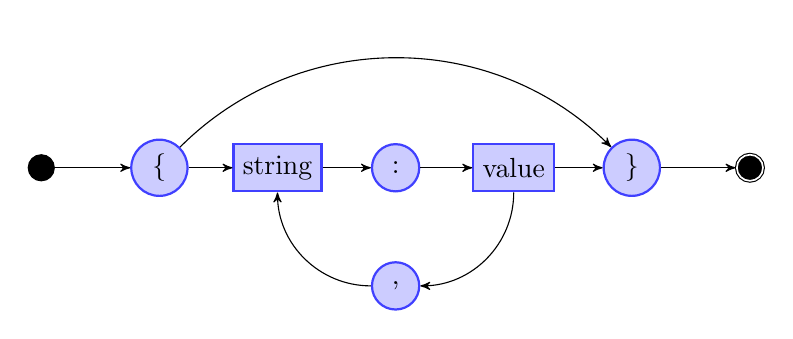
\begin{tikzpicture}[node distance=1.5cm,>=stealth',bend angle=45,auto]
  \tikzset{initial text=$ $,
              ->}
  \tikzstyle{literal}=[state,thick,draw=blue!75,fill=blue!20,minimum size=6mm]
  \tikzstyle{rule}=[rectangle,thick,draw=blue!75,fill=blue!20,minimum size=6mm]

  \tikzstyle{every label}=[red]
    \node [literal] (lbrack)                                    {\{};
    \node [state, draw=black, fill=black, minimum size=3mm] (initial) [left of=lbrack] {};
    \node [rule] (string)  [right of=lbrack]                               {string};
    \node [literal] (colon) [right of=string] {:};
    \node [rule] (value) [right of=colon] {value};
    \node [literal] (rbrack) [right of=value] {\}};
    \node [literal] (comma) [below of=colon] {,};
    \node [state, accepting, draw=black, fill=black, minimum size=3mm] (final) [right of=rbrack] {};

   \draw (initial) edge (lbrack)
            (lbrack) edge (string)
            (lbrack) edge[bend left, above] (rbrack)
            (string) edge (colon)
            (colon) edge (value)
            (value) edge (rbrack)
            (rbrack) edge (final)
            (value) edge[bend left, below] (comma)
            (comma) edge[bend left, below] (string) ;

\end{tikzpicture}
\end{center}
\end{frame}

\begin{frame}
\frametitle{JSON Array}
\begin{center}
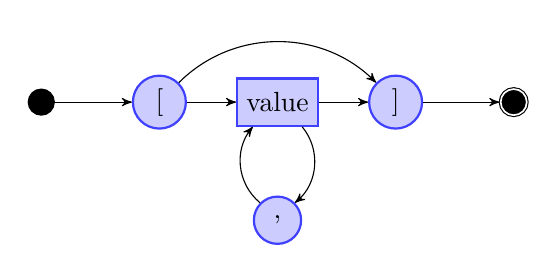
\begin{tikzpicture}[node distance=1.5cm,>=stealth',bend angle=45,auto]
  \tikzset{initial text=$ $,
              ->}
  \tikzstyle{literal}=[state,thick,draw=blue!75,fill=blue!20,minimum size=6mm]
  \tikzstyle{rule}=[rectangle,thick,draw=blue!75,fill=blue!20,minimum size=6mm]

  \tikzstyle{every label}=[red]
    \node [literal] (lbrack)                                    {[};
    \node [state, draw=black, fill=black, minimum size=3mm] (initial) [left of=lbrack] {};
    \node [rule] (value) [right of=lbrack] {value};
    \node [literal] (rbrack) [right of=value] {]};
    \node [literal] (comma) [below of=value] {,};
    \node [state, accepting, draw=black, fill=black, minimum size=3mm] (final) [right of=rbrack] {};

   \draw (initial) edge (lbrack) 
            (lbrack) edge (value)
            (lbrack) edge[bend left, above] (rbrack)
            (value) edge (rbrack)
            (rbrack) edge (final)
            (value) edge[bend left, below] (comma)
            (comma) edge[bend left, below] (value) ;

\end{tikzpicture}
\end{center}
\end{frame}

\begin{frame}
\frametitle{JSON Value}
\begin{center}
\scalebox{0.7}{
\begin{tikzpicture}[node distance=1.3cm,>=stealth',bend angle=45,auto]
  \tikzset{initial text=$ $,
              ->}
  \tikzstyle{literal}=[state,thick,draw=blue!75,fill=blue!20,minimum size=6mm]
  \tikzstyle{rule}=[rectangle,thick,draw=blue!75,fill=blue!20,minimum size=6mm]

  \tikzstyle{every label}=[red]

    \node [state, draw=black, fill=black, minimum size=3mm] (initial)  {};

    \node [rule] (array) [right of=initial] {array};
    \node [rule] (object) [above of=array] {object};
    \node [rule] (number) [above of=object] {number};
    \node [rule] (string) [above of=number] {string};
    \node [literal] (true) [below of=array] {true};
    \node [literal] (false) [below of=true] {false};
    \node [literal] (null) [below of=false] {null};
    \node [state, accepting, draw=black, fill=black, minimum size=3mm] (final) [right of=rbrack] {};

   \draw (initial) edge  [bend left, above]  (string)
            (initial) edge   [bend left, above]  (number)
            (initial) edge [bend left, above] (object)
            (initial) edge (array)
            (initial) edge [bend right] (true)
            (initial) edge [bend right] (false)
            (initial) edge [bend right] (null)
            (string) edge [bend left] (final)
            (number) edge [bend left] (final)
            (object) edge [bend left] (final)
            (array) edge  (final)
            (true) edge [bend right] (final)
            (false) edge [bend right] (final)
             (null) edge [bend right] (final);

\end{tikzpicture}
}
\end{center}
\end{frame}

\begin{frame}
\frametitle{JSON String}
We will use a heavily simplified version of the string for now.
\begin{center}
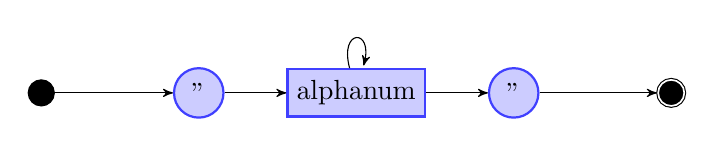
\begin{tikzpicture}[node distance=2cm,>=stealth',bend angle=45,auto]
  \tikzset{initial text=$ $,
              ->}
  \tikzstyle{literal}=[state,thick,draw=blue!75,fill=blue!20,minimum size=6mm]
  \tikzstyle{rule}=[rectangle,thick,draw=blue!75,fill=blue!20,minimum size=6mm]

  \tikzstyle{every label}=[red]

    \node [state, draw=black, fill=black, minimum size=3mm] (initial)  {};

    \node [literal] (leftquote) [right of=initial] {"};
    \node [rule] (alphanum) [right of=leftquote] {alphanum};
    \node [literal] (rightquote) [right of=alphanum] {"};
   \node [state, accepting, draw=black, fill=black, minimum size=3mm] (final) [right of=rightquote] {};

   \draw (initial) edge  (leftquote)
            (leftquote) edge (alphanum)
            (alphanum) edge (rightquote)
            (rightquote) edge (final)
            (alphanum) edge [loop above] (alphanum);

\end{tikzpicture}
\end{center}
\end{frame}


\begin{frame}
\frametitle{JSON Number}
We also use a heavily simplified version of the number.
\begin{center}
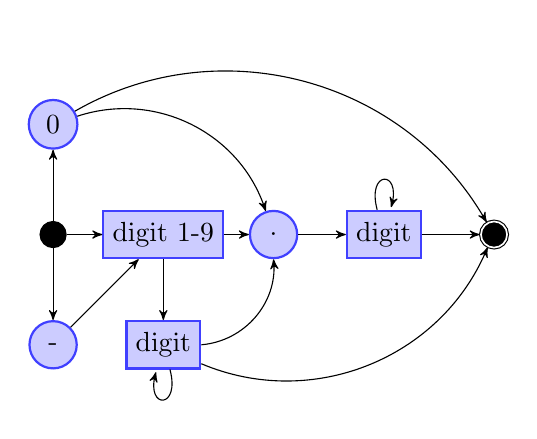
\begin{tikzpicture}[node distance=1.4cm,>=stealth',bend angle=45,auto]
  \tikzset{initial text=$ $,
              ->}
  \tikzstyle{literal}=[state,thick,draw=blue!75,fill=blue!20,minimum size=6mm]
  \tikzstyle{rule}=[rectangle,thick,draw=blue!75,fill=blue!20,minimum size=6mm]

  \tikzstyle{every label}=[red]

    \node [state, draw=black, fill=black, minimum size=3mm] (initial)  {};

    \node [literal] (minus) [below of=initial] {-};
    \node [rule] (onetonine) [right of=initial] {digit 1-9};
    \node [literal] (zero) [above of=initial] {0};
    \node [literal] (dot) [right of=onetonine] {.};
    \node [rule] (digit1) [below of=onetonine] {digit};
    \node [rule] (digit2) [right of=dot] {digit};
    \node [state, accepting, draw=black, fill=black, minimum size=3mm] (final) [right of=digit2] {};

   \draw (initial) edge (zero)
            (initial) edge (onetonine)
            (initial) edge (minus)
            (minus) edge (onetonine)
            (onetonine) edge (digit1)
            (digit1) edge [loop below] (digitone)
            (zero) edge [bend left] (final)
            (zero) edge [bend left] (dot)
            (onetonine) edge (dot)
            (dot) edge (digit2)
            (digit2) edge (final)
            (digit1) edge [bend right] (dot)
            (digit1) edge [bend right] (final)
            (digit2) edge [loop above] (digit2);

\end{tikzpicture}
\end{center}
\end{frame}


\begin{frame}[fragile]
\frametitle{Exercise 2 Create a JSON Parser: Task 1}
Create a parser for JSON \textbf{strings} using the following grammar:
\medskip
\begin{grammar}
<string> ::= "<alphanum>"
\end{grammar}

\end{frame}


\begin{frame}[fragile]
\frametitle{Exercise 2 Create a JSON Parser: Task 2}
Create a parser for JSON \textbf{numbers} using the following grammar:
\medskip
\begin{grammar}
<number> ::= <int> <frac>

<int> ::=  <digit> | <onenine> <digits> | - <digit> | - <onenine><digits>

<frac> ::= "" | . <digits>

<digits> ::= <digit> | <digit> <digits>

<digit> ::= 0 | <onenine>

<onenine> ::= 1-9
\end{grammar}

\end{frame}


\begin{frame}[fragile]
\frametitle{Exercise 2 Create a JSON Parser: Task 3}
Create a parser for JSON \textbf{values} using the following grammar:
\medskip
\begin{grammar}
<value> ::= <object> | <array> | <string> | <number> | true | false | null
\end{grammar}
\end{frame}

\begin{frame}[fragile]
\frametitle{Exercise 2 Create a JSON Parser: Task 4}
Create a parser for JSON \textbf{arrays} using the following grammar:
\medskip
\begin{grammar}
<array> ::= [] | [ <values> ]

<values> ::= <value> | <value> , <values>
\end{grammar}
\end{frame}


\begin{frame}[fragile]
\frametitle{Exercise 2 Create a JSON Parser: Task 5}
Create a parser for JSON \textbf{objects} using the following grammar:
\medskip
\begin{grammar}
<object> ::= \{ \} | \{ <members> \}

<members> ::= <member> | <member> , <members>

<member> ::= <string> : <value>
\end{grammar}
\end{frame}


\begin{frame}[fragile]
\frametitle{Dealing with Whitespace}
By default Pyparsing parsers automatically consume whitespace. \\
\medskip
It is possible to change this by using the \texttt{setDefaultWhitespaceChars} method e.g. \\
\medskip
\begin{verbatim}
ParserElement.setDefaultWhitespaceChars("\t")
\end{verbatim}
\bigskip
See example \textbf{whitespace.py}.

\end{frame}


\begin{frame}[fragile]
\frametitle{Exercise 2 Create a JSON Parser: Task 6}
Extend our JSON string parser to deal with escaped characters \escape{t} and \escape{n}.
\end{frame}


\begin{frame}
\frametitle{Packrat Parsing}
An optimization technique for parsers. 

\begin{verbatim}

\end{verbatim}

Disabled by default.
\end{frame}


\begin{frame}
\frametitle{Packrat Parsing}
How does this work? It uses a technique called \textbf{memoization} or \textbf{tabling}

\begin{verbatim}

\end{verbatim}

Disabled by default.
\end{frame}

\begin{frame}
\frametitle{Tracing Parsers}
\end{frame}

\begin{frame}
\begin{center}
Thats the end of the workshop. Thanks for listening.
\end{center}
\end{frame}

\end{document}


\begin{frame}
\frametitle{Intermediate Pyparsing}

\end{frame}



\begin{frame}
\frametitle{Lookahead with NotAny and FollowedBy}
\end{frame}

\begin{frame}
\frametitle{Parsing dictionaries with Dict}
\end{frame}


\begin{frame}
\frametitle{Forward declaring parsers with Forward}
\end{frame}


\begin{frame}
\frametitle{Exercise 2: JSON Parser}
\end{frame}

\begin{frame}
\frametitle{Advanced Pyparsing}
\end{frame}


\begin{frame}
\frametitle{Debugging parsers}
\end{frame}

\begin{frame}
\frametitle{Whitespace Management}
\end{frame}


\begin{frame}
\frametitle{Packrat Parsing}
An optimization technique for parsers. 

\begin{verbatim}

\end{verbatim}

Disabled by default.
\end{frame}

\begin{frame}
\frametitle{Packrat Parsing}
An optimization technique for parsers. 

\begin{verbatim}

\end{verbatim}

Disabled by default.
\end{frame}


\begin{frame}
\frametitle{Summary}
\end{frame}


\end{document}
